\chapter[Use Cases]{Use Cases}\label{cap:use_cases}

In the present chapter we are going to test the UQMS in three different scenarios, spatial only domain, section \ref{Wave Propagation} , spatio-temporal domain, section \ref{spatio_temporal}, and finally a multidisciplinary system, section \ref{NASA}. 

\section{Case Study:  Wave Propagation Problem}\label{Wave Propagation}

\subsection{The Dataset}
In the HPC4e benchmark, the models have been designed as a set of 16 layers with constant physical properties. The top layer delineates the topography and the other 15 delineate different layer interface surfaces or horizons. To generate a single cube with dimensions $250\times501\times501$ we can use the values provided in the benchmark. For example, to generate a cube in the $v_{p}(m/s)$ variable we can use the fixed values of Table \ref{tab:valuesOfVp}.

\begin{table}
\begin{center}
    \begin{tabular}{|l|l|}
    \hline
    \textbf{Layer} & $v_{p}(m/s)$ \\ \hline
    1     & 1618.92 \\ \hline
    2     & 1684.08 \\ \hline
    3     & 1994.35 \\ \hline
    4     & 2209.71 \\ \hline
    5     & 2305.55 \\ \hline
    6     & 2360.95 \\ \hline
    7     & 2381.95 \\ \hline
    8     & 2223.41 \\ \hline
    9     & 2712.06 \\ \hline
    10    & 2532.22 \\ \hline
    11    & 2841.03 \\ \hline
    12    & 3169.31 \\ \hline
    13    & 3252.35 \\ \hline
    14    & 3642.28 \\ \hline
    15    & 3659.22 \\ \hline
    16    & 4000.00 \\ \hline
    \end{tabular}
    \caption {Values of $v_{p}$ used in the generation of a single velocity field cube.}
    \label{tab:valuesOfVp}
    \end{center}
\end{table}
The first slice of this cube is shown in Figure \ref{fig:slice1}.

\begin{figure}[H]
    \centering
    \includegraphics[width=0.8\textwidth]{images/velocity_field.png}
    \caption{One slice of the $250\times501\times501$ cube. In the slice we can distinguish between the different layers.}
    \label{fig:slice1}
\end{figure}

Now as our purpose is to study the uncertainty in the output as a result of the propagation of the input uncertainty throughout the model, we cannot use this benchmark as it is. We need the input, $v_{p}(m/s)$  in this case, to be uncertain. In order to achieve so, we compute $v_{p}(m/s)$ as a random variable with the \textit{PDFs} shown in Table \ref{tab:PDFsOfVp}.

\begin{table}
\begin{center}
    \begin{tabular}{|l|l|l|}
    \hline
    \textbf{Layer} & \textbf{PDF Family}                & \textbf{Parameters}           \\ \hline
    1     & Gaussian & [1619, 711.2] \\ \hline
    2     & Gaussian & [3368, 711.2]               \\ \hline
    3     & Gaussian & [8839, 711.2]               \\ \hline
    4     & Gaussian & [7698, 301.5]               \\ \hline
    5     & Lognormal   & [7723, 294.7]               \\ \hline
    6     & Lognormal   & [7733, 292.2]               \\ \hline
    7     & Lognormal   & [7658, 312.1]               \\ \hline
    8     & Lognormal   & [3687, 368.7]               \\ \hline
    9     & Exponential & [3949, 394.9]             \\ \hline
    10   & Exponential & [5983, 711.2]               \\ \hline
    11   & Exponential & [3520, 352.0]              \\ \hline
    12   & Exponential & [3155, 315.5]              \\ \hline
    13   & Uniform     & [2541, 396.4]              \\ \hline
    14   & Uniform     & [2931, 435.3]              \\ \hline
    15   & Uniform     & [2948, 437.0]             \\ \hline
    16   & Uniform     & [3289, 471.1]              \\ \hline
    \end{tabular}
    \caption {PDFs and its parameteres used to sampling the $v_{p}$, to generate n velocity models.}
    \label{tab:PDFsOfVp}
    \end{center}
\end{table}

Then, using a Monte Carlo method we generate a sampling of 1000 realizations of the $v_{p}(m/s)$ variable, Figure \ref{fig:vp_1000_realizations}; and using a Matlab script provided by the HPC4e benchmark we simulate 1000 times, one for each  realization, and generate 1000 cubes (230 GB) as an output. The resulting cubes are $250\times501\times501$  multi-dimensional arrays. 

\begin{figure}[ht]
    \centering
    \includegraphics[width=0.8\textwidth]{images/vp_1000_realizations.png}
    \caption{Histograms of the 1000 samplings generated using Monte Carlo method and the PDFs reported in Table \ref{tab:PDFsOfVp}.}
    \label{fig:vp_1000_realizations}
\end{figure}

To simplify the computational process and visualize the results, we select the slice 200 to be used here, then we have 1000 realizations of a slice with size of $250\times501$. The equation \ref{eq:data_base_structure} can be simplified because we have two dimensions in space and don't have time domain, then our dataset can be represented as $S(x_{i},y_{j},simId,v_{p}(x_{i},y_{j}))$. In this new representation $(x_{i},y_{j})$ are the 2D coordinates and $v_{p}(x_{i},y_{j})$ is the velocity value at point $(x_{i},y_{j})$. \textit{simId} still represents the Id of the simulation and its range here is between 1 and 1000.

Now that we have an experimental dataset we can start to apply our workflow, step by step.

\subsection{Fitting the GLD}
The first step is to find the \textit{GLD} that best fits the dataset at each spatial location. Running the algorithm proposed in Section \ref{gldFitProcess} we get as a result a new 2D array:
\begin{equation}\label{eq:gld_fit_2D}
S'(x_{i},y_{j},GLD(\lambda_{1}, \lambda_{2}, \lambda_{3}, \lambda_{4}))
\end{equation}
The raw data is reduced and our dataset is characterized by four lambda values at each spatial location. Now we need to assess the validity of the \textit{GLDs} and how well they fit the dataset. Those analyses are described in sections \ref{useCaseGLDValidityCheck} and \ref{useCaseQualityofFit}. 

\subsection{GLD validity check}\label{useCaseGLDValidityCheck}
Once the algorithm to check the validity of the \textit{GLD} is run on the experimental dataset, we obtain as a result that the \textit{GLD} is valid in all the $(x_{i},y_{j})$ space.

\subsection{Quality of the fit}\label{useCaseQualityofFit}
The next step is to check how good is the fit. To do this we use an algorithm that returns the \textit{D} and \textit{p-value} for the KS-test at each spatial location. As we show in figure \ref{fig:p_value}, and remember that with a \textit{p-value} $>0.05$ we cannot reject the null hypothesis, we conclude that the fit of the GLD is acceptable in most cases. To be more exact, the p-value was greater than 0.05 in 82 \% of the spatial locations, figure \ref{fig:p_values_greater_05}.

\begin{figure}[H]
    \centering
    \includegraphics[width=0.8\textwidth]{images/p_value.png}
    \caption{Goodness of the fit based on the \textit{p}-value returning by the KS-test. \textit{p}-value $>$ 0.05 represent a good fit of the GLD to the dataset at $(x_{i}, y_{j})$.}
    \label{fig:p_value}
\end{figure}

\begin{figure}[H]
    \centering
    \includegraphics[width=0.8\textwidth]{images/p_value_greater_05.png}
    \caption{The red color shows where the p-value was greater than 0.05.}
    \label{fig:p_values_greater_05}
\end{figure}

If we consider the distance \textit{D}, returned by the KS-test, the result is similar, figure \ref{fig:kolmogorov_distance}. We can see a blue region that is common in figures \ref{fig:p_values_greater_05} and \ref{fig:kolmogorov_distance}. This region is where the quality of the GLD fit is below a threshold. 
%In order to understand what happens in this region, we manually analyze some spatial points inside it. The result is shown in Figure 53. In fact, all the points we analyzed presented the same behavior as the one depicted in Figure 53, modelled as an exponential distribution. Visually, the fit looks good but the KS-test is suggesting a different situation. 
On those cases, some \textit{GLD} extensions proposed in \cite{Karian2011} could be used.

As the main purpose of this paper is to demonstrate the utility of the use of the \textit{GLD} in \textit{UQ}, then we are not going to deep in other algorithms to solve this particular problem.

\begin{figure}[H]
    \centering
    \includegraphics[width=0.8\textwidth]{images/kolmogorov_distance.png}
    \caption{Kolmogorov-Smirnoff Distance (D). The red regions represent where the GLD fits well.}
    \label{fig:kolmogorov_distance}
\end{figure}

\subsection{Clustering}\label{useCaseClustering}
At this point we have our dataset characterized by the schema depicted by Equation \ref{eq:gld_fit_2D}, then using a clustering algorithm, such as k-means, we are going to group the GLDs based on its $(\lambda_{2}, \lambda_{3}, \lambda_{4})$ values, as those are the values that describe the shape of the distribution at each point of the dataset.

In this paper we use k-means algorithm with $n=10$, where $n$ is the number of clusters to be made. This is an arbitrary value, we are investigating other algorithms as DBSCAN and what are the $\epsilon$ of this algorithm that warranty a good clusterization, but discussing alternative GLDs clustering algorithms is beyond the scope of this paper.

Once the clustering algorithm has been applied, a new dataset is produced, where for each spatial location we have a label that indicates the cluster the GLD at each position belongs to (see the schema at Equation \ref{eq:clustersresult}), Figure \ref{fig:clusters}. Note that, in Figure \ref{fig:clusters}, the blue region corresponding to cluster 11 is not a cluster itself. It is rather the region where the \textit{GLD} is not valid, see section \ref{useCaseQualityofFit}.

\begin{equation}\label{eq:clustersresult}
S_{\mathcal{C}}(x_{i},y_{j},clusterID, GLD_{x_{i},y_{j}})
\end{equation}

\begin{figure}[H]
    \centering
    \includegraphics[width=0.8\textwidth]{images/clusters1.png}
    \caption{Result of the clusterization using k-means with $n=10$.}
    \label{fig:clusters}
\end{figure}

If we visually compare Figure \ref{fig:slice1} with Figure \ref{fig:clusters}, we observe a close similarity between the two. It is clear that they can not be equal because we are talking about a slice of a deterministic model, and the result of making clusters on 1000 realizations of a stochastic model, but as the model used here is very linear, this is the result we expect.

Another interesting result is shown in Figure \ref{fig:clusters_lambda3_lambda4_space}, where we plot the clusters in $(\lambda_{3}, \lambda_{4})$ space. As we mention in section \ref{gldShape}, the shape of the \textit{GLD} depends on the values of $\lambda_{3}$ and $\lambda_{4}$. In this scenario, the expected result is that the members of the same cluster share similar values of $\lambda_{3}$ and $\lambda_{4}$. This is exactly the result we can observe in Figure \ref{fig:clusters_lambda3_lambda4_space}. 

\begin{figure}[H]
    \centering
    \includegraphics[width=0.8\textwidth]{images/Clusters_lambda3_lambda4.png}
    \caption{Distribution of the clusters in the $(\lambda_{3}, \lambda_{4})$ space. The points that belongs to a same cluster are one near the others, as was expected.}
    \label{fig:clusters_lambda3_lambda4_space}
\end{figure}

To further corroborate this fact, in Figure \ref{fig:cluster1} we show the \textit{PDFs} of 60 members of the 10 clusters. Visually assessing the figures we have an idea of how similar are the shapes of the members of a same cluster and how dissimilar are the shapes of the  members of different clusters. This suggests that our approach is valid. A product of these observations is that we can pick one member of each cluster (the centroid) as a representative of all the members of this cluster, Table \ref{tab:center_of_the_clusters}. The selected member is going to be used to answer the queries in the next sections.

\begin{figure}[ht]
    \centering
    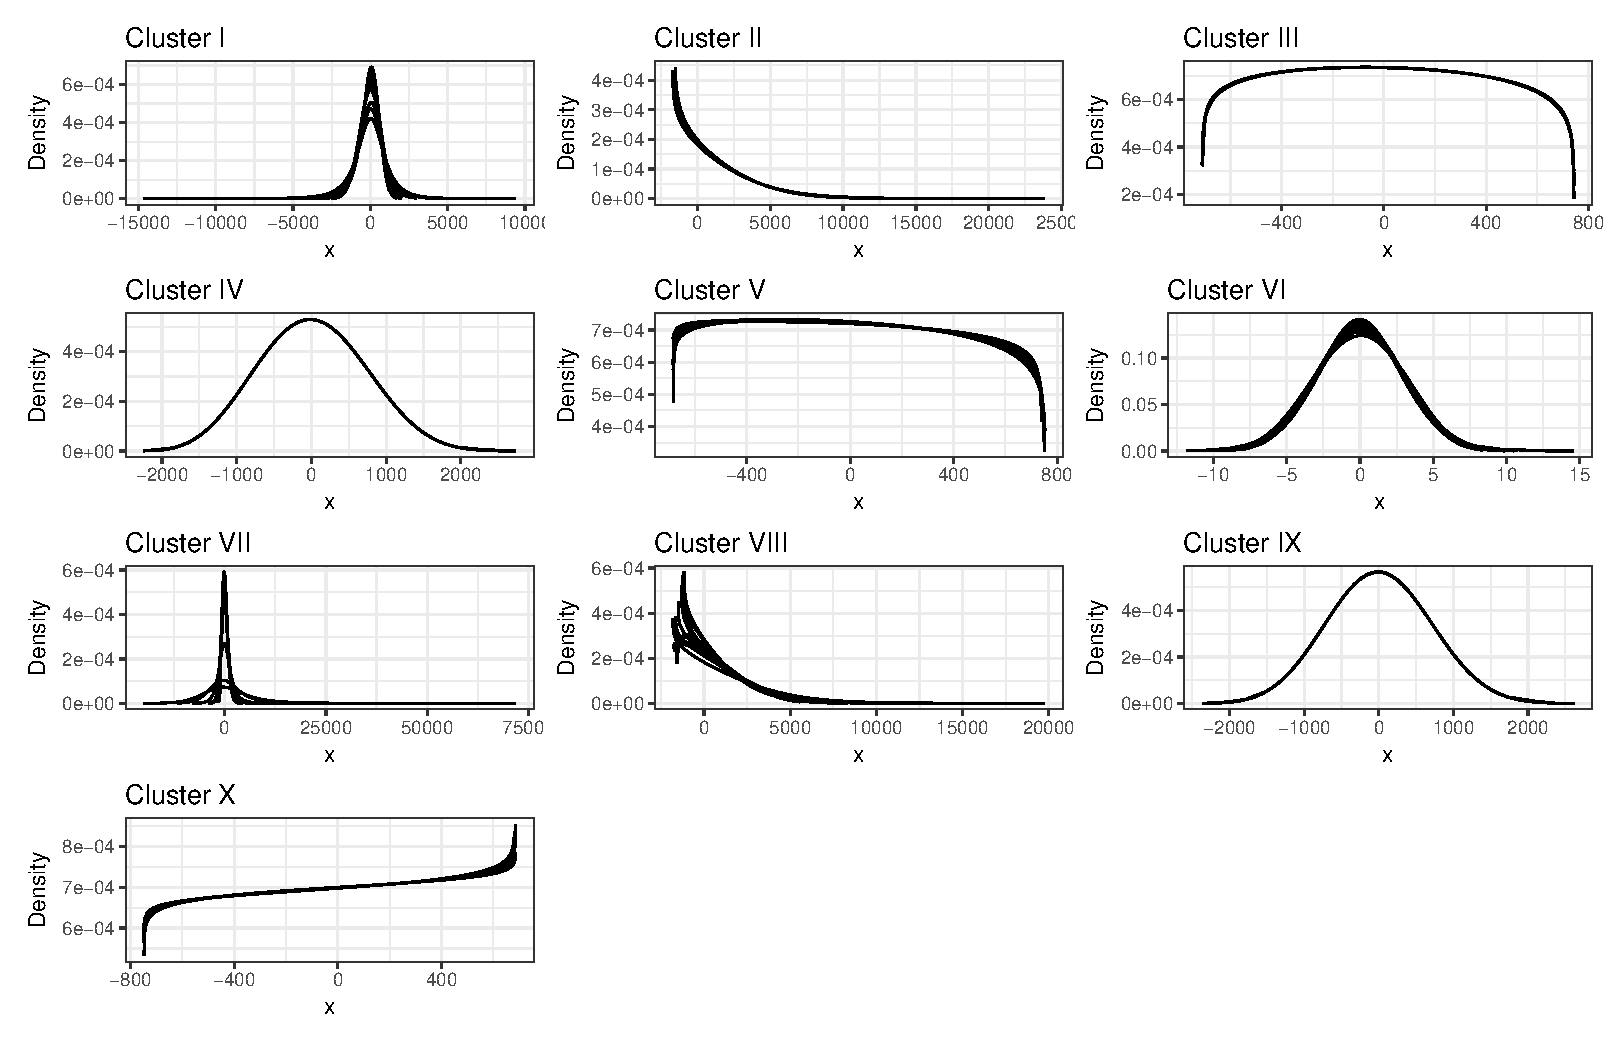
\includegraphics[width=\textwidth]{img/use_cases/clusters.eps}
    \caption{\textit{PDFs} of 60 members of the 10 clusters obtained using k-means over the $(\lambda_{2}, \lambda_{3}, \lambda_{4})$ values.}
    \label{fig:cluster1}
\end{figure}

\begin{table}
\begin{center}
    \begin{tabular}{|l|l|l|l|}
    \hline
    \textbf{Cluster} & $\lambda_{2}$ & $\lambda_{3}$ & $\lambda_{4}$         \\ \hline
    1     & 0.0013937313 & 0.9585829 & 1.04696461              \\ \hline
    2     & 0.0005291388 & 1.1633978 & -0.07162550            \\ \hline
    3     & 0.0020630696 & 0.1349486 & 0.17305941            \\ \hline
    4     &  0.0016238358 & 0.8653824 & 0.83857646               \\ \hline
    5     & 0.0027346929 & 0.5084664 & 0.39199164                \\ \hline
    6     & 0.0003894541 & 1.4076354 & -0.01925743               \\ \hline
    7     & 0.0021972784 & 0.3253562 & 0.01493809                 \\ \hline
    8     & 0.0015421749 & 0.9491101 & 0.86699555                \\ \hline
    9     & 0.0018672401 & 0.2176002 & 0.17862024            \\ \hline
    10   & 0.4856397733 & 0.1404140 & 0.14011298             \\ \hline
    \end{tabular}
    \caption {Centers of the clusters.}
    \label{tab:center_of_the_clusters}
    \end{center}
\end{table}

The 125250 points of the slice are distributed through the clusters following the histogram of the figure \ref{fig:Clusters_histogram} and Table \ref{tab:distribution_of_the_clusters}. 

\begin{figure}[H]
    \centering
    \includegraphics[width=0.8\textwidth]{images/Clusters_histogram.png}
    \caption{Distribution of the clusters.}
    \label{fig:Clusters_histogram}
\end{figure}

\begin{table}
\begin{center}
    \begin{tabular}{|l|l|l|}
    \hline
    \textbf{Cluster} & \textbf{No. of members}         \\ \hline
    1     & 27217              \\ \hline
    2     & 15223             \\ \hline
    3     & 6749            \\ \hline
    4     & 3421               \\ \hline
    5     & 1353                \\ \hline
    6     & 25853               \\ \hline
    7     & 1374                 \\ \hline
    8     & 18103                 \\ \hline
    9     & 12051            \\ \hline
    10   & 13156              \\ \hline
    \end{tabular}
    \caption {Distribution of the clusters.}
    \label{tab:distribution_of_the_clusters}
    \end{center}
\end{table}

\subsection{Spatio-temporal queries}\label{spatio_temporal_queries}
At this point, the initial dataset is summarized as depicted by the schema in equation \ref{eq:clustersresult}. It can be used to answer queries and to validate our approach, comparing the results with the raw data.

First of all we select four spatio-temporal regions of the dataset where the clusters suggest us different behaviors. The regions are shown in Figure \ref{fig:analysis_regions} and the values of $[x_{1}, x_{2}], [y_{1}, y_{2}]$ that define the regions are shown in Table \ref{tab:analysis_regions}. 

\begin{figure}[H]
    \centering
    \includegraphics[width=0.8\textwidth]{images/regions.png}
    \caption{Analysis Regions.}
    \label{fig:analysis_regions}
\end{figure}

\begin{table}
\begin{center}
    \begin{tabular}{|l|l|l|l|l|}
    \hline
    \textbf{Region} & $x_{1}$ & $x_{2}$ & $y_{1}$ & $y_{2}$        \\ \hline
    Region 1     & 210 & 250 & 0 & 40              \\ \hline
    Region 2     & 150 & 250 & 50 & 150           \\ \hline
    Region 3     & 0 & 75 & 100 & 200            \\ \hline
    Region 4     & 0 & 250 & 300 & 400               \\ \hline
    \end{tabular}
    \caption {Analysis Regions.}
    \label{tab:analysis_regions}
    \end{center}
\end{table}

With these four regions we assess the adoption of the \textit{GLD} mixture to obtain the \textit{PDF} that characterizes the uncertainty in an specific  region, section \ref{GLDmixtureresults}; and in section \ref{informationEntropyresults}. We use the Information Entropy to assign a value that measures the uncertainty at each region. In section \ref{GLDmixtureresults}, we expect the GLD mixture to characterize well the raw data; and in \ref{informationEntropyresults} we hope that the information entropy is zero in region 1 and increases between regions 2, 3 and 4.

\subsubsection{GLD mixture}\label{GLDmixtureresults}
The experiment here is to use the representative \textit{GLDs} at each cluster and the weight associated to it in the region. Using these parameters we can build a \textit{GLD mixture} that characterizes the uncertainty on that region. Here we use the algorithm described in section \ref{GLDMixture}.

First of all we query the region to find  the clusters represented inside it, and how are they distributed. Below we show the R codes to query the four regions. The retrieved results are shown in Table \ref{tab:distribution_of_the_clusters_by_regions}.

\begin{lstlisting}[language=R]
> clRegion1 = clByRegion(210, 250, 0, 40)
> clRegion2 = clByRegion(150, 250, 50, 150)
> clRegion3 = clByRegion(0, 75, 100, 200)
> clRegion4 = clByRegion(0, 250, 300, 400)
\end{lstlisting}

\begin{table}
\begin{center}
    \begin{tabular}{|l|l|l|l|l|}
    \hline
    \textbf{Cluster} & \textbf{Region 1} &  \textbf{Region 2} &  \textbf{Region 3} &   \textbf{Region 4}  \\ \hline
    1     & 0   		& 2250 & 0 & 979            \\ \hline
    2     & 0   		& 0 & 0 & 268           \\ \hline
    3     & 0      	& 0 & 2596 & 1468       \\ \hline
    4     & 1640	& 4467 & 0 & 5173         \\ \hline
    5     & 0       & 149 & 0 & 269          \\ \hline
    6     & 0     & 0 & 0 & 416           \\ \hline
    7     & 0       & 0 & 1967 & 3920           \\ \hline
    8     & 0     & 3335 & 0 & 3432             \\ \hline
    9     & 0      & 0 & 1918 & 3280       \\ \hline
    10   & 0      & 0 & 901 & 583         \\ \hline
    \end{tabular}
    \caption {Distribution of the clusters by regions.}
    \label{tab:distribution_of_the_clusters_by_regions}
    \end{center}
\end{table}

If we divide the columns of Table \ref{tab:distribution_of_the_clusters_by_regions} by the sum of the elements of each column we get the weight needed to formulate the \textit{mixed GLDs}. It is clear that the \textit{GLD} in region 1 is represented by the \textit{GLD} of cluster 4. On the other 3 cases we get:

\begin{equation*}\label{eq:pareto mle2}
  \begin{aligned}
& GLD_{region1} = GLD_{c4} \\
& GLD_{region2} = 0.22GLD_{c1} + 0.44GLD_{c4} + 0.014GLD_{c5} \\
& + 0.33GLD_{c8} \\
& GLD_{region3} = 0.34GLD_{c3} + 0.26GLD_{c7} + 0.25GLD_{c9} \\
& + 0.12GLD_{c10} \\
& GLD_{region4} = 0.22GLD_{c1} + 0.44GLD_{c4} + 0.014GLD_{c5} \\ 
& + 0.33GLD_{c8}
\end{aligned}
\end{equation*}

Now we need to evaluate if the \textit{mixture of GLDs} describes well the uncertainty in the regions. To do this we perform the same \textit{ks-test} used to evaluate the goodness of the fit and described in Section \ref{Quality of the fit}. 

\begin{table}
\begin{center}
    \begin{tabular}{|l|l|l|l|l|}
    \hline
    \textbf{Metrics} & \textbf{Region 1} &  \textbf{Region 2} &  \textbf{Region 3} &   \textbf{Region 4}  \\ \hline
    p-value     & 0.73   		& 0.56 & 0.34 & 0.08            \\ \hline
    \end{tabular}
    \caption {p-values by regions.}
    \label{tab:p_values_by_regions}
    \end{center}
\end{table}

Based on the \textit{p-value}, Table \ref{tab:p_values_by_regions}, we can conclude that in all 4 regions the \textit{mixture of GLDs} is a good fit to the raw data.

\subsubsection{Information Entropy}\label{informationEntropyresults}
Now we are going to evaluate what happens with the information entropy. Based on the distribution of clusters inside the regions, table \ref{tab:distribution_of_the_clusters_by_regions}; we can compute the entropy. In this case we use an R function called \textit{entropy}, implemented in the r-package of the same name  \cite{Hausser2008}.

\begin{table}
\begin{center}
    \begin{tabular}{|l|l|l|l|l|}
    \hline
    \textbf{entropy} & \textbf{Region 1} &  \textbf{Region 2} &  \textbf{Region 3} &   \textbf{Region 4}  \\ \hline
    value     & 0   		& 1.122243 & 1.41166 & 2.024246            \\ \hline
    \end{tabular}
    \caption {Information Entropy by regions.}
    \label{tab:entropy_by_regions}
    \end{center}
\end{table}

As we expect, Table \ref{tab:entropy_by_regions}, the entropy in region 1 is zero, because the region contains only members of the cluster 4. On the other regions the entropy increases from region 2 to region 4, as we expected.

It is clear that the information entropy is a very good and simple measure of the uncertainty, and here it is demonstrated its utility combined with the \textit{GLD}.

The first one is a geophysical tests for wave propagation problems

As a first case study we use the “HPC4E Seismic Test Suite”, a collection of four 3D models and sixteen associated tests that can be downloaded freely at the project's website (https://hpc4e.eu/downloads/datasets-and-software ). The models include simple cases that can be used in the development stage of any geophysical imaging practitioner (developer, tester ...) as well as extremely large cases that can only be solved in a reasonable time using ExaFLOPS supercomputers. The models are generated to the required size by means of a Matlab/Octave script and hence can be used by users of any OS or computing platform. The tests can be used to benchmark and compare the capabilities of different and innovative seismic modelling approaches, hence simplifying the task of assessing the algorithmic and computational advantages that they pose. %\cite{deLaPuente2015}

In our case, we are going to use the “HPC4E Seismic Test Suite” as a case study of the porposed UQMS. As we mention in the introduction of this chapter this model is a spatial only domain problem, because we are going to consider a multidimentional array as an Input and a multidimentional array as an output, but of them time independet.

\subsection{Mathematical Formulation}

\subsection{Model and Dataset Description}
The models have been designed as a set of 16 layers with constant physical properties. The top layer delineates the topography and the other 15 different layer interface surfaces or horizons. In the following, an interface horizon is associated with properties that apply to the layer that exists between itself and the immediately next layer horizon. The model covers an area of 10 x 10 x 5 km, with maximum topography at about 500 m and maximum depth at about 4500 m. The layer horizons have been sampled very finely with 1.6667 m spacing so that a highly accurate representation can be honored at high frequencies. For simulation schemes based on unstructured grids, the layer horizons can be used easily to constrain model blocks. For simulation schemes based upon Cartesian grids, a simple script is provided that can generate 3D grids for any desired spatial sampling. Table \ref{layers_constants} shows the properties of each of the layers included in the models. %\cite{deLaPuente2015}

\begin{table}[]
\centering
\caption{Layer constant properties and their depth range. “Star” layers are only used in the flat case, in substitution of their non-star equivalents}
\label{layers_constants}
\begin{tabular}{|l|l|l|l|l|l|}
\hline
\multicolumn{1}{|c|}{\textbf{\begin{tabular}[c]{@{}c@{}}Layer\\ Id\end{tabular}}} & \multicolumn{1}{c|}{\textbf{\begin{tabular}[c]{@{}c@{}}Vp\\ (m/s)\end{tabular}}} & \multicolumn{1}{c|}{\textbf{\begin{tabular}[c]{@{}c@{}}Vs\\ (m/s)\end{tabular}}} & \multicolumn{1}{c|}{\textbf{\begin{tabular}[c]{@{}c@{}}Density\\ (Kg/m3)\end{tabular}}} & \multicolumn{1}{c|}{\textbf{\begin{tabular}[c]{@{}c@{}}Max. depth\\ (m)\end{tabular}}} & \multicolumn{1}{c|}{\textbf{\begin{tabular}[c]{@{}c@{}}Min. depth\\ (m)\end{tabular}}} \\ \hline
1 & 1618.92 & 500.00 & 1966.38 & -135.55 & -476.35 \\ \hline
2 & 1684.08 & 765.49 & 1985.88 & 41.50 &  -394.90 \\ \hline
3 &  &  &  &  &  \\ \hline
4 &  &  &  &  &  \\ \hline
5 &  &  &  &  &  \\ \hline
6 &  &  &  &  &  \\ \hline
7 &  &  &  &  &  \\ \hline
8 &  &  &  &  &  \\ \hline
9 &  &  &  &  &  \\ \hline
10 &  &  &  &  &  \\ \hline
11 &  &  &  &  &  \\ \hline
12 &  &  &  &  &  \\ \hline
13 &  &  &  &  &  \\ \hline
14 &  &  &  &  &  \\ \hline
15 &  &  &  &  &  \\ \hline
16 &  &  &  &  &  \\ \hline
2* &  &  &  &  &  \\ \hline
3* &  &  &  &  &  \\ \hline
\end{tabular}
\end{table}

\subsection{Adding uncertainty into the model}

The “HPC4E Seismic Test Suite” does not provide uncertainty sources, because all the input parameters of the model have fixed values. Then, to the purpose of our work we need to add some uncertainties into the inputs. Let's suppose the variable ${V_{p}}$ is uncertain. As this variable have 16 different values, one for each layer, we can consider it as a random vector, equation \ref{random_vector_vp}. We associate to each of the $V_{{p}_{i}}$ a Normal distribution with ${\mu}_{i}$ equal to the value reported in Table \ref{layers_constants} and $\sigma=2$.
\begin{equation}\label{random_vector_vp}
V_{p}=<V_{{p}_{i}},\mathcal{N}({\mu}_{i},{\sigma}_{i})>
\end{equation}

\section{Case study with cross-correlated variables}
Este caso de estudio es el primero del paquete R spup. Nuestros resultados son los mismos que ellos muestran haciendo uso de la GLD. Una query interesante es encontrar donde determinado valor es mayor que 24. En los codigos del capitulo esta la respuesta super facil haciendo uso de la funcion qgl del paquete GLDEX. Esta funcion nos devuelve el valor del quantil 90 y de ahi buscamos donde este valor es mayor que 30, el resultado es el mismo que ellos muestran en el ejemplo.

\section{Case Study: Austin, queso library}\label{spatio_temporal}

\section{Case Study: Multidisciplinary System (NASA)}\label{NASA}

\section{Case Study: Spatio-temporal Nicholson-Bailey model}
Este esta en el software uqlab, en la carpeta Doc Manuals
